

In \exrange{exercise-3.1.1}{exercise-3.1.4}, write each quadratic function in standard form. Then determine whether its graph will open up or open down without graphing the function.


\begin{exercise}\label{exercise-3.1.1}
$f(x)=x(4x-7)$
\end{exercise}

\begin{solution}
    $f(x)=4x^2-7x$; opens up
\end{solution}





\begin{exercise}
$h(t)=17+3t-5t^2-2(1.5t-2)$
\end{exercise}

\begin{solution}
    $h(t)=-5t^2+21$; opens down
\end{solution}





\begin{exercise}
$g(x)=4x(x-4)-2x(x-1)$
\end{exercise}

\begin{solution}
    $g(x)=2x^2-14x$; opens up
\end{solution}





\begin{exercise}\label{exercise-3.1.4}
$y=-4(x+5)^2+80$
\end{exercise}

\begin{solution}
     $y=-4x^2-40x-20$; opens down
\end{solution}






\noindent In \exrange{exercise-3.1.5}{exercise-3.1.6}, use the graph of each quadratic function to identify its intercept(s) and vertex.

\begin{exercise}\label{exercise-3.1.5}

\begin{center}
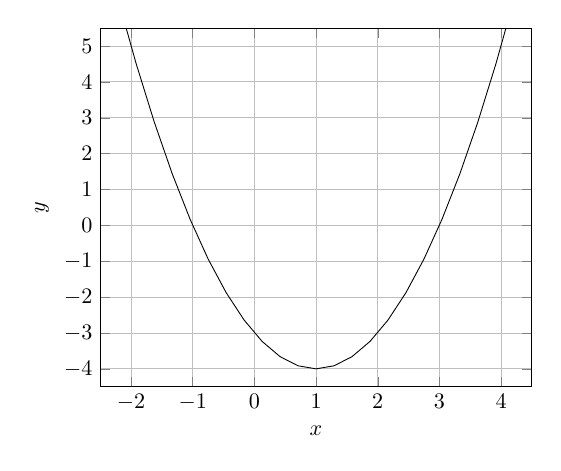
\begin{tikzpicture}[scale=0.8]
\begin{axis}[grid=both,
xmin=-2.5,xmax=4.5,
ymin=-4.5,ymax=5.5,
xtick={-2,...,4},
ytick={-4,...,5},
minor tick={},
xlabel=\(x\), ylabel=\(y\),
]
\addplot[domain=-2.5:4.5] {(x+1)*(x-3)};
\end{axis}
\end{tikzpicture}
\end{center}
\end{exercise}

\begin{solution}
     horizontal intercepts: $-1$, $3$; vertical intercept: $-3$; vertex: $(1,-4)$
\end{solution}






\begin{exercise}\label{exercise-3.1.6}
\begin{center}
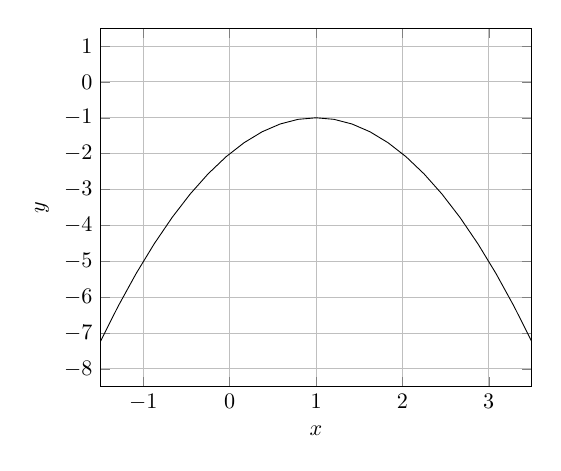
\begin{tikzpicture}[scale=0.8]
\begin{axis}[grid=both,
xmin=-1.5,xmax=3.5,
ymin=-8.5,ymax=1.5,
xtick={-2,...,4},
ytick={-8,...,5},
minor tick={},
xlabel=\(x\), ylabel=\(y\),
]
\addplot[domain=-1.5:3.5] {-(x-1)^2-1};
\end{axis}
\end{tikzpicture}
\end{center}
\end{exercise}

\begin{solution}
    no horizontal intercepts; vertical intercept: $-2$; vertex: $(1,-1)$
\end{solution}









\noindent In \exrange{exercise-3.1.7}{exercise-3.1.8}, the horizontal intercepts of a quadratic parabola are given. Find the $x$-coordinate of its vertex.



\begin{exercise}\label{exercise-3.1.7}$\displaystyle x=-1.5 \mbox{ and } x=1.5$
\end{exercise}

\begin{solution}
    $0$
\end{solution}





\begin{exercise}\label{exercise-3.1.8}$\displaystyle x=-2 \mbox{ and } x=5$
\end{exercise}

\begin{solution}
    $\frac{3}{2}$
\end{solution}





\begin{exercise} A quadratic parabola crosses the $x$-axis at the point $(2,0)$ and has its vertex at the point $(4,4)$. Find the second point on the $x$-axis where the parabola crosses the $x$-axis. Does the parabola open up or open down?
\end{exercise}

\begin{solution}
    $(6,0)$; opens down
\end{solution}



\begin{exercise} A lighting company can sell $1000-2p$ units of its specialty chandelier if it charges \$$p$ per specialty chandelier.
\begin{parts}
\item Find the formula for the revenue $R(p)$ generated from specialty chandelier sales and graph it.
\item At what price will the lighting company sell zero of its specialty chandelier?
\item What is the maximum revenue? What price should the lighting company charge per specialty chandelier in order to maximize revenue?
\end{parts}
\end{exercise}

\begin{solution}
    \begin{parts}
        \item $R(p)=p(1000-2p)$ or $R(p)=-2p^2+1000p$
        \item $\$500$
        \item The maximum revenue is \$125,000. The lighting company should charge $\$250$ per specialty chandelier to maximize revenue.
    \end{parts}
\end{solution}